%%%%%%%%%%%%%%%%%%%%%%%%%%%%%%%%%%%%%%%%%%%%%%%%%%%%%%%%%%%%%%%%%%%%%%%%%%%%%%%%%%%%%%%%%%%%%%%%%%%%%%%%%%%%%%%%%%%%%%%%%
\subsection{NoWA: SSD WAF=1 on Commodity SSDs}\label{sec:nowa}
With a single active zone, achieving SSD WAF~\(=1\) is straightforward (\cref{fig:gcunit0}).  
With multithreading, however, multiple zones are appended simultaneously, which complicates the problem.
In this section, we explain how WA arises from \emph{multiplexing} and \emph{frequency imbalance} among zones within the same active group~\cite{flashalloc}.  
We then introduce the NoWA write pattern, which prevents SSD-GC-induced WA and thereby guarantees SSD WAF~\(=1\) on commodity SSDs.  
For FDP-enabled SSDs, multiplexing can be avoided without NoWA; we discuss this in the next section.

\begin{figure}[t]
    \centering
    %--- First figure ---
    \begin{minipage}[b]{0.49\linewidth}
        \centering
          \setlength{\abovecaptionskip}{3pt} % space above caption
        \setlength{\belowcaptionskip}{0pt} % space below caption (usually inside float)
        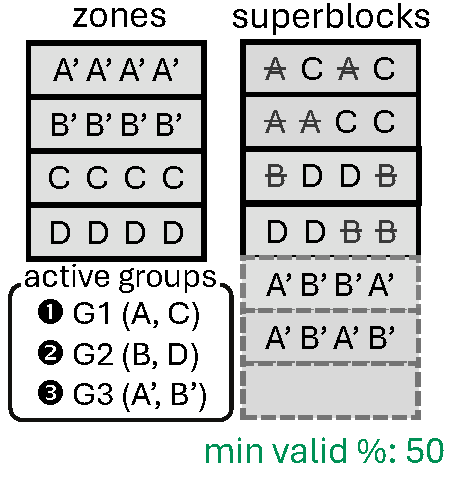
\includegraphics[width=0.7\linewidth]{figures/frequencyimbalance.pdf}
        \caption{Imbalanced frequency in active groups}
        \label{fig:multipleopen}
    \end{minipage}
    \hfill
    %--- Second figure ---
    \begin{minipage}[b]{0.49\linewidth}
        \centering
          \setlength{\abovecaptionskip}{3pt} % space above caption
  \setlength{\belowcaptionskip}{0pt} % space below caption (usually inside float)
        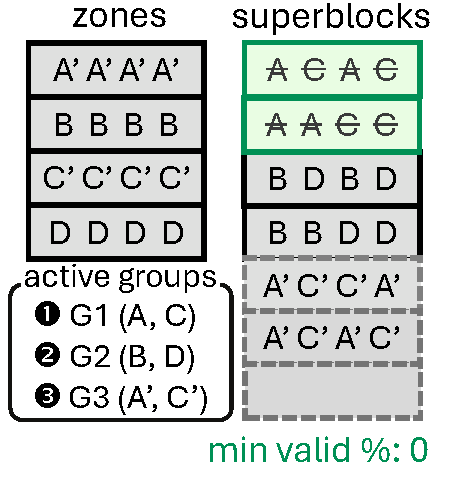
\includegraphics[width=0.7\linewidth]{figures/nofrequencyimbalance.pdf}
        \caption{No frequency imbalance in active groups}
        \label{fig:noimbalance}
    \end{minipage}
\end{figure}


\module{Multiplexing occurs with multiple open zones.}
When multiple zones are appended concurrently, their write streams interleave across different superblocks~\cite{purandare2025valet}.
For example, if the DBMS writes to zones A and C at the same time (active group G1(A, C) in \cref{fig:multipleopen}), 
writes from both zones become mixed, scattering their data across two superblocks.
This multiplexing effect~\cite{flashalloc} arises because standard SSDs cannot distinguish writes from zone A and C.

\module{Frequency imbalance in an active group incurs WA.}
Multiplexing causes WA when zones in the same active group are invalidated at different rates.
In \cref{fig:multipleopen}, selecting zones A and B for DB GC (active group G3(A', B')) produces four partially invalidated superblocks that the SSD GC must later rewrite.
If, however, all zones in the active group are invalidated uniformly, the SSD can still produce superblocks with a 0\% valid-page ratio even under multiplexing.
For example, choosing G(A', C') in \cref{fig:noimbalance} fully invalidates two superblocks.
Thus, balanced invalidation within an active group eliminates SSD WA even when writes are multiplexed across zones.

\module{Optimization: NoWA pattern guarantees SSD WAF of 1.}
The \emph{NoWA pattern} eliminates SSD-GC--induced WA by ensuring that the SSD always has at least one fully invalidated superblock available when it reaches its minimum free--superblock threshold.
NoWA achieves this by estimating how pages are multiplexed within the SSD’s physical layout and enforcing two rules:
(1) defer opening new zones until all currently open zones are completely written, and
(2) detect and correct write--frequency imbalances among concurrently appended zones.
By selecting DB-GC victim zones in accordance with these principles, NoWA guarantees the existence of an empty superblock before SSD GC is triggered.
In effect, this write pattern preempts SSD-level GC.

\module{NoWA properties.}
The key idea behind NoWA is to eliminate frequency imbalance \emph{before} SSD GC is triggered.
As shown in \cref{fig:multipleopen}, if a new active group (e.g., G3(A', B')) creates uneven invalidation in earlier groups (e.g., A:2 vs.\ C:1 in G1),
the DBMS issues a \emph{compensation write} for the underrepresented zone (e.g., CW(C)), as illustrated in \cref{fig:nowa}.
This compensation must occur before the SSD reaches its minimum free--space threshold, which can be estimated using SSD--iq~\cite{ssdiq}.
The compensation write recompacts the scattered pages of zone~C into a single superblock, invalidating their older versions and effectively producing two fully invalidated superblocks.
Thus, NoWA proactively restores balance whenever imbalance occurs, ensuring that subsequent SSD GC cycles operate on fully invalidated superblocks.

\begin{figure}[t]
    \centering

    %--- First figure ---
    \begin{minipage}[b]{0.42\linewidth}
        \centering
          \setlength{\abovecaptionskip}{3pt} % space above caption
  \setlength{\belowcaptionskip}{0pt} % space below caption (usually inside float)
        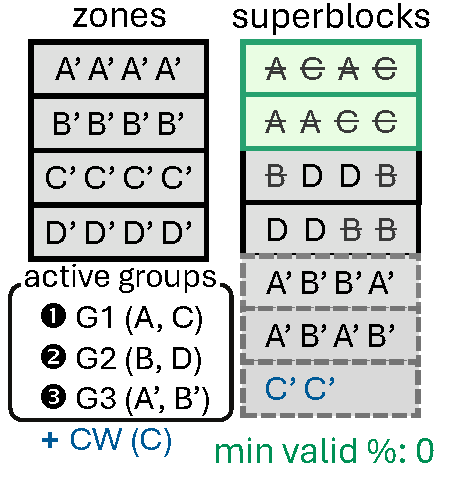
\includegraphics[width=0.8\linewidth]{figures/nowa.pdf}
        \caption{NoWA's compensation writes}
        \label{fig:nowa}
        \vspace{-3mm} 
    \end{minipage}
    \hfill
    %--- Second figure ---
    \begin{minipage}[b]{0.54\linewidth}
        \centering
          \setlength{\abovecaptionskip}{3pt} % space above caption
  \setlength{\belowcaptionskip}{0pt} % space below caption (usually inside float)
        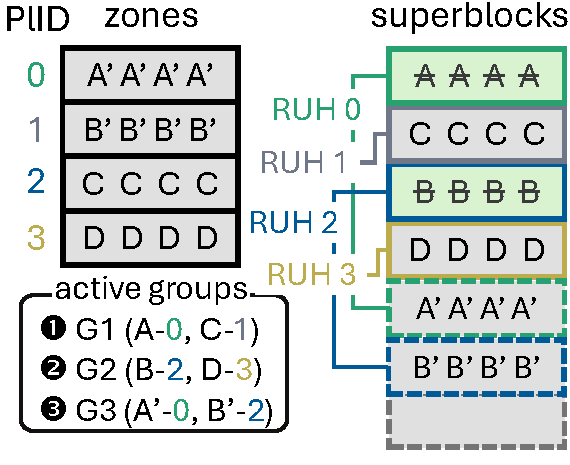
\includegraphics[width=0.8\linewidth]{figures/fdp.pdf}
        \caption{FDP placement hints avoid multiplexing}
        \label{fig:fdp}
        \vspace{-3mm} 
    \end{minipage}
\end{figure}

\module{Compensation writes are not entirely redundant.}
Compensation writes shift a small portion of WA from the SSD to DBMS-level GC.
Although they increase DB WAF slightly, the overhead is modest because the DBMS controls zone selection.
Before selecting a victim zone, GC can check whether issuing a compensation write would raise valid-page ratios in later rounds; if so, it simply chooses another zone.
Overall, this small increase in DB WAF is far outweighed by the reduction in SSD WAF (e.g., from 2.3 in in-place to 1 with out-of-place LeanStore using NoWA; see \cref{fig:intro}).

\module{Flexible zone sizing with NoWA.}
NoWA also allows flexible configuration of DB zone size by adjusting the maximum number of concurrently open zones.
NoWA holds as long as $\mathrm{max\ open\ zones} \times \mathrm{zone\ size}$
equals or is a multiple of the inferred SSD GC unit.
For example, on FDP-enabled SSD~A, 16 active zones of 513~MB each, or 8 zones of 1{,}026~MB, satisfy this requirement.
This flexibility enables smaller zones to reduce GC-induced tail latency while preserving NoWA’s guarantee of SSD WAF~=~1.

\module{NoWA is worthwhile, even if it is imperfect.}
\revision[R2.D11]{NoWA may not always completely eliminate SSD WA, 
since SSDs may reorder or relocate data depending on scheduling, load, flash chip state, open-superblock limits, or wear-leveling~\cite{lerner2024principles}. 
However, it still provides substantial practical benefit: even partial mitigation of page mixing reduces WA.
Nevertheless, NoWA achieves SSD WAF~=~1 on six enterprise SSDs from diverse vendors and capacities (\cref{fig:varyingssd}).}
